% Template for ICASSP-2016 paper; to be used with:
%          spconf.sty  - ICASSP/ICIP LaTeX style file, and
%          IEEEbib.bst - IEEE bibliography style file.
% --------------------------------------------------------------------------
\documentclass[12pt]{article}
\usepackage{spconf, amsmath, graphicx, float}
\usepackage{scrlayer-scrpage}
\clearpairofpagestyles
\cfoot*{\pagemark}
% Example definitions.
% --------------------
\def\x{{\mathbf x}}
\def\L{{\cal L}}

% Title.
% ------
\title{Movie Review Sentiment Analysis}
%
% Single address.
% ---------------
\name{{\bf Atom Group}: Jifu Zhao (jzhao59), Jinsheng Wang (jwang278)}
\address{Nuclear, Plasma, and Radiological Engineering \\
              University of Illinois at Urbana-Champaign\\
		       Urbana, Illinois 61801, USA}

\begin{document}
%\ninept
%
\maketitle

\section{Introduction}
\quad\ In this project, our goal is to build a model to predict the chance of default for a loan. The data is collected through the Lending Club. The original data set has more than 130,000 records and each record has 74 features. In this project, we first explore the given training data set. After some pre-processing methods, we applied several different models to predict the chance of default for a loan. More details will be described in the following sections.

\section{Pre-processing}
After exploring the training dataset, we noticed that there are 74 features in total. Among these 74 features, we first notice that feature $id$ and $member\_id$ are useless. Among other features, we also notice that features $mths\_since\_last\_delinq$, $ max\_bal\_bc $, $ all\_util $, $ total\_cu\_tl $, $ mths\_since\_last\_record$, \\$ mths\_since\_last\_major\_derog $, $ annual\_inc\_joint $, $ dti\_joint $, $ open\_acc\_6m $, $ open\_il\_6m $, $ inq\_last\_12m $, $ open\_il\_12m $, $ open\_il\_24m $, $ il\_util $, $ inq\_fi $, \\$ mths\_since\_rcnt\_il $, $ total\_bal\_il $, $ open\_rv\_12m $, $ open\_rv\_24m $ contains too many missing values, so we first drop these features.

In addition to these features, we also notice that some features are useless, including $emp\_title$, $issue\_d$, $pymnt\_plan$, $url$, $desc$, $title$, $zip\_code$, $addr\_state$, $earliest\_cr\_line$, $last\_pymnt\_d$, \\$next\_pymnt\_d$, $last\_credit\_pull\_d$, $application\_type$, $verification\_status\_joint$, $grade$, $policy\_code$. Besides, since the order of $sub\_grade$ make sense, we directly transform it into numerical values. Then, for missing values, we fill them with the median of the corresponding feature in the training set. And for the $loan\_staus$ feature, we transform it into 0-1 value.

After the above procedures, there are 36 features left. Among these 36 features, there are 30 numerical features and 6 categorical features. For categorical features, we transform them into dummy variables. For numerical variables, for those whose skewness is above 0.75, we choose the log transformation. After all of these steps, we have prepared the data set to train some classification models.

In our R code, we loaded 6 libraries to simplify our task, including xgboost, randomForest, gbm, dummies, DAAG, glmnet.


\section{Methods}

\subsection{Logistic Regression with Ridge Penalty}
In our first model, Model 1, we basically choose the nearby three weeks to make prediction. For example, for a given store and department in week w, we find the corresponding data for the same department and store from the last year, then we choose the median of the sales from w - 1, w, w + 1 as the prediction.

\subsection{Logistic Regression with Lasso Penalty}

\subsection{Multinomial Naive Bayes Model}

\subsection{AdaBoost}

\subsection{Gradient Boosting}
In this model, considering the long running time, we choose the weighted average of Model 1 and Model 2 as our third model, Model 3. Through some careful study, we find the the weight should be 0.7 for Model 1 and 0.3 for Model 2. The final expression for Model 3 is shown below:


\subsection{Random Forest}
In Method 2, we choose ts() to create a time series whose frequency is 52 and auto.arima() to forecast for a give step. More specially, for a given store and department, we first extract the data from previous years that is from the same department and store. Then we use the ts() function to create a time series whose frequency is 52. Finally, through feeding the time series into auto.arima(), we make the prediction that corresponding to next month's sales.





\section{Code Description}
\quad\ All of our code is contained in the file named mymain.R. 


There are basically three parts in the R file. At the very beginning, the code will automatically check whether or not the required packages/libraries are already installed. In the second part of the code, we do data preprocessing: first read the training and test data sets, then drop the useless variables and process the features to form the new feature space. For the last part, we mainly build our three model: Linear Regression, Lasso Regression and Random Forest model. These built models will make predictions and the results are saved into local file system as required by the project description.

Due to the amount of data to be looped, the code need a lot of time to run. As tested, the total running time is around 2 hours.

\section{Results}

To evaluate our model, we choose the metric described on Kaggle:
\begin{equation}
logloss = - \frac{1}{N} \sum_{i=1}^N \sum_{j=1}^M y_{i, j} log(p_{i, j})
\end{equation}
where $N$ is the number of test cases, $M$ is the total classification classes. To avoid the problem where $p_{i, j} = 0$, we scale $p_{i, j}$ into $10 ^ {-15}$ and $1 - 10 ^ {-15}$.


\begin{table}[htb]
 \caption{Summary of Training Loss} \label{result}
 \vspace{0.1in}
\begin{center}
  \begin{tabular}{  c  c  c  c  c}
    \hline
    Split            & Seed        & Model 1    & Model 2    & Model 3 \\ \hline
    Split 1         & 100    \\ \hline
    Split 2         & 500    \\ \hline
    Split 3         & 1000    \\ \hline
    Split 4         & 5000    \\ \hline
    Split 5         & 2017    \\ \hline
  \end{tabular}
\end{center}
\end{table}

\begin{table}[htb]
 \caption{Summary of Test Loss} \label{result}
 \vspace{0.1in}
\begin{center}
  \begin{tabular}{  c  c  c  c  c}
    \hline
    Split            & Seed        & Model 1    & Model 2    & Model 3 \\ \hline
    Split 1         & 100    \\ \hline
    Split 2         & 500    \\ \hline
    Split 3         & 1000    \\ \hline
    Split 4         & 5000    \\ \hline
    Split 5         & 2017    \\ \hline
  \end{tabular}
\end{center}
\end{table}


From Table~\ref{result}, one can find that, Model 1 and Model 2 performs similar to each other. Through weighted averaging, the final model, Model 3, performs better than Model 1 and Model 2.

The above code is tested on our laptop, the average running time is about 6 hours. The corresponding computer system is:
MacBook Pro, 2.6GHz Intel Core i7, 16 GB memory.  

\subsection*{Acknowledgement}

%\begin{figure}[htb]
%\centering
%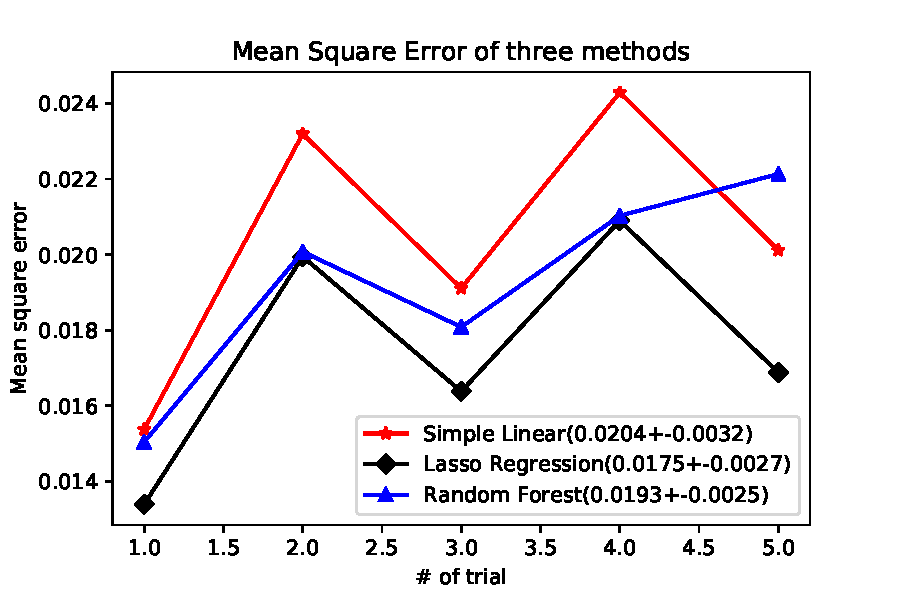
\includegraphics[width=0.45\textwidth]{./figures/MSE_3_methods.pdf}
%\caption{Results of different models}
%\label{fig:autoencoder}
%\end{figure}

\quad\ The authors would like to thank Xichen Huang for his tutorial notebook on Piazza and David Thaler for his online code.

\vfill\pagebreak

% References should be produced using the bibtex program from suitable
% BiBTeX files (here: strings, refs, manuals). The IEEEbib.bst bibliography
% style file from IEEE produces unsorted bibliography list.
% -------------------------------------------------------------------------
%\bibliographystyle{IEEEbib}%\bibliography{strings,refs}
%\bibliography{strings}

\end{document}